\course{Base de datos de profesores}
\professor{Juan Baldelomar}

\maketitle

\part{Bitácora}
%%_2 de febrero_%%
\begin{entry}{2 de febrero}
\tcbsubtitle{\LBlimportant}
\begin{itemize}
    \item Artículo en \href{https://medium.com/codex/principal-component-analysis-pca-how-it-works-mathematically-d5de4c7138e6}{Medium} sobre \textit{PCA}.
    \begin{itemize}
        \item Procedimiento matemático
        \item Procedimiento programático
    \end{itemize}
    
    \item Artículo de \href{https://towardsdatascience.com/understanding-pca-fae3e243731d}{Towards datascience}, \textit{Understanding PCA}.
    \begin{itemize}
        \item Importancia de \textit{PCA}
        \item Conjunto ideal
        \item Pérdida de sentido
    \end{itemize}
\end{itemize}
\tcblower
\tcbsubtitle{\LBlsummary}
Con el artículo de Medium conseguí entender como es el funcionamiento matemático de \textit{PCA}. Este consiste en reducir la dimensión de los vectores de datos que tenemos en nuestro modelo. Esto se consigue calculando el producto punto de cada vector de dato con los \textit{Eigen vectors} de la matriz de covarianza de los datos estandarizados. El procedimiento matemático y programático se encuentra mejor desarrollado en la sección \ref{PCAmath}, parte \ref{Notas}.\\

En el artículo de Towards datascience explican que la importancia detrás de la reducción dimensional radica en evitar el \textit{overfitting} en nuestro modelo cuando la cantidad de \textit{features} es muy grande relativo a la cantidad de \textit{samples}. Además de eso nos describieron como es el conjunto ideal de \textit{features}
\begin{itemize}
    \item Con alta varianza
    \item Poca correlacionadas
    \item No muchas
\end{itemize}
Sin embargo los ejemplos dados en ese artículo (\textit{100 Days of Stock Returns for 30 Different Stocks}) no me parecen muy triviales, pero creo que la manera de verlo correctamente sería graficando la rentavilidad de cada día como un eje (\textit{feature}) y cada empresa sería un vector en la gráfica (\textit{sample}). Así que el \textit{PCA} combinaría distintas rentabilidades.\\

Un contra del \textit{PCA} es que perdemos certeza de que significan las \textit{feature}.
%\vspace{0.4em}
\tcbsubtitle{\LBltodo}\vspace{-1.25em}
\begin{itemize}
    \item ¿Que son los estimadores de varianza/desviación estándar, \textbf{sesgados} y \textbf{no sesgados}?
    
    \item ¿Es correcta mi interpretación del ejemplo en el artículo de Towards datascience?
    \end{itemize}
\end{entry}

\begin{entry}{2 de febrero}
\tcbsubtitle{\LBlimportant}
\begin{itemize}
    \item Vídeos de YouTube de StatQuest
    \begin{itemize}
        \item \href{https://youtu.be/FgakZw6K1QQ}{Vídeo largo}
        \item \href{https://youtu.be/HMOI_lkzW08}{Vídeo corto}
    \end{itemize}
    \item Artículo \href{https://www.javatpoint.com/principal-component-analysis#:~:text=Principal\%20Component\%20Analysis\%20is\%20an,the\%20help\%20of\%20orthogonal\%20transformation}{Javatpoint}
    \begin{itemize}
        \item Aplicaciones de \textit{PCA}
    \end{itemize}
\end{itemize}
\tcblower
\tcbsubtitle{\LBlsummary}
Las visualizaciones del vídeo largo de StatQuest me ayudaron a entender mejor como proyectar datos a dimensiones distintas de uno, cosa que no tenia demasiado claro. Además de introducir la idea del \textit{clustering} y su significado.\\

Lo que no entiendo muy bien es por que la transformación lineal que se mapea a la matriz de covarianza tiene como \textit{eigen vectors} las dimensiones con mayor varianza (creo que alli me falta un poco de entendimiento que me tiene algo confundido).\\

En el vídeo largo también se explicó que es un \textit{scree plot}, que es el grafico de barras que se enseñó en la lectura de Medium (puede verse en \ref{PCAmath-scree}) y con eso podremos ver que tan certera es la representación de nuestro \textit{PCA}.\\

Las visualizaciones del vídeo corto me parecen confusas.\\

El artículo de Javatpoint lo pude leer con más calma, pues siento que allí pude corroborar la mayoría de lo que pensaba de \textit{PCA}, me interesó particularmente que dijeran que se podía usar \textit{PCA} en el sistema de recomendación de películas, ya que me interesaría ver si con un \textit{dataset} que encontré en Kaggle (\href{https://www.kaggle.com/hernan4444/anime-recommendation-database-2020?select=anime.csv}{Anime Recommendation Database 2020}) se podría hacer algo similar (aunque ahorita mismo no estoy muy seguro de ciertos puntos).
\vspace{0.4em}
\tcbsubtitle{\LBltodo}\vspace{-1.25em}
\begin{itemize}
    \item ¿Posible confusión entre \textit{features} y \textit{samples} en el video corto de StatQuest?
\end{itemize}
\end{entry}

%%_9 de febrero_%%
\begin{entry}{9 de febrero}
\tcbsubtitle{\LBlimportant}
\begin{itemize}
    \item \textit{PCA} aplicado al \textit{dataset} de \href{https://scikit-learn.org/stable/modules/generated/sklearn.datasets.load_wine.html}{\textit{Wine recognition}}
\end{itemize}
\tcblower
\tcbsubtitle{\LBlsummary}
Aunque técnicamente trabajé el \textit{dataset} la semana del 2 de febrero, aproveché que la semana pasada la pasé casi en su totalidad leyendo para separarlo así.\\

El estudio de la base de de datos de vino no trajo consigo resultados satisfactorios, quería ver si era posible distinguir los tipos de vino utilizando la reducción dimensional de \textit{PCA} a 2 dimensiones, sin embargo la poca cantidad de varianza representada ($55.41\%$) hace imposible hacer una distinción suficientemente clara. Para tratar de tener una visualización más clara (solo por diversión) programé una visualización en 3D, pero lamentablemente su cantidad de varianza sigue siendo muy baja ($66.53\%$).\\

Se puede ver tódo el código en ...
\vspace{0.4em}
\tcbsubtitle{\LBltodo}\vspace{-1.25em}
\begin{itemize}
    \item ¿Cuánta varianza es óptima para \textbf{visualización}?
    \item Buscar más \textit{datasets} en los que se vea bien \textit{PCA}.
\end{itemize}
\end{entry}

\begin{entry}{9 de febrero}
\tcbsubtitle{\LBlimportant}
\begin{itemize}
    \item Mi propia implementación de \textit{PCA} (\texttt{MyPCA.py}).
\end{itemize}
\tcblower
\tcbsubtitle{\LBlsummary}
Hice la implementación de \textit{PCA} revisando al mismo tiempo cosas de la sección \ref{PCAmath} de este documento, como leyendo el artículo de Javatpoint. Realicé la implementación con \textit{OOP} y luego la probé en Jupyter Lab contra el \textit{PCA} de \texttt{sklearn}.
\vspace{0.4em}
\tcbsubtitle{\LBltodo}\vspace{-1.25em}
\begin{itemize}
    \item Tengo que documentar al menos un poco \texttt{MyPCA.py} solo para que sea medianamente legible.
\end{itemize}
\end{entry}

\newpage%%%%%%%%%%%%%%%%%%%%%%%%%%%%%%%%%%%%%%%%%%%%%%%%%%%%%%%%%

\part{Notas adicionales} \label{Notas}
\section{Matemáticas de \textit{PCA}}\label{PCAmath}
En esta sección trataré de hacer una comparación paso a paso y lado a lado del procedimiento manual para hacer \textit{PCA} y como hacerlo de manera automatizada con Python (Todo el procedimiento y código está basado en el artículo original de Medium, ver en la entrada correspondiente al 4 de febrero).
\subsection{Pasos preliminares}
Para trabajar con Python ejecute esos comandos desde la primera celda del \textit{Jupyter notebook}, \textit{Jupyter lab} o desde el editor de su elección.
\begin{jupyter}{1}
import numpy as np
import pandas as pd
import matplotlib.pyplot as plt
from sklearn.decomposition import PCA
\end{jupyter}
Considerese el \textit{dataset} siguiente, con 2 columnas (\textit{features}) y 6 filas (\textit{samples}).
\begin{table}[H]
\centering
\begin{tabular}{cc}
\sffamily X & \sffamily Y \\ 
\hline
\rowcolor[HTML]{EFEFEF} 
2 & 3 \\
4 & 5 \\
\rowcolor[HTML]{EFEFEF} 
6 & 5 \\
6 & 7 \\
\rowcolor[HTML]{EFEFEF} 
7 & 8 \\
5 & 8
\end{tabular}
\caption{\textit{dataset}}\label{tab:PCAmath-dataset}
\end{table}
Notese que los pares $(2,3)$, $(4,5)$, $(6,5)$, $(6,7)$, $(7,8)$, $(5,8)$ son llamados \textit{feature vectors}.\\

Estos datos se introducirán a Python con
\begin{jupyter}{2}
data = np.array([[2,3],[4,5],[6,5],[6,7],[7,8],[5,8]])
df = pd.DataFrame(data=data, columns=['X', 'Y'])
df
\end{jupyter}
que nos devolverá la misma tabla \ref{tab:PCAmath-dataset}.

\subsection{Normalizar datos}
\begin{minipage}[c]{0.48\textwidth}
Calculamos la media de los datos
\[ \overline{\mathsf{X}}=5 \qquad \overline{\mathsf{Y}}=6, \]
desviación estándar (con estimador de varianza sesgado)
\[ S_{\mathsf{X}}=1.633 \qquad S_{\mathsf{Y}}=1.826, \]
y aplicaremos a cada valor de $\mathsf{X}$ y $\mathsf{Y}$, la formula:
\[ Z=\frac{\mathsf{X}_i-\overline{\mathsf{X}}}{S_{\mathsf{X}}} \]
\end{minipage}
\hfill\vrule\hfill
\begin{minipage}[c]{0.48\textwidth}
\begin{jupyter}{3}
from scipy.stats import zscore
df_scaled = df.apply(zscore)
print("Scaled Data:")
df_scaled
\end{jupyter}
\end{minipage}\\

lo que resulta en:
\begin{table}[H]
\centering
\begin{tabular}{cc}
\sffamily X & \sffamily Y \\
\hline
\rowcolor[HTML]{EFEFEF} 
$-1.837$ & $-1.643$ \\
$-0.612$ & $-0.548$ \\
\rowcolor[HTML]{EFEFEF} 
$0.612$ & $-0.548$  \\
$0.612$ & $0.548$   \\
\rowcolor[HTML]{EFEFEF} 
$1.225$ & $1.095$   \\
$0$     & $1.095$
\end{tabular}
\caption{Salida estandarizada (mismo resultado en ambas aproximando a 3 decimales)}
\label{tab:PCAmath-standarized}
\end{table}

\subsection{Matriz de covarianza}
\begin{minipage}[c]{0.48\textwidth}
Para sacar la matiz de covarianza calcularemos:
\begin{equation*}
\begin{bmatrix}
\cov(\mathsf{X},\mathsf{X}) & \cov(\mathsf{X},\mathsf{Y})\\
\cov(\mathsf{Y},\mathsf{X}) & \cov(\mathsf{Y},\mathsf{Y})
\end{bmatrix}
=
\begin{bmatrix}
1.2 & 0.939\\
0.939 & 1.2
\end{bmatrix}
\end{equation*}
\end{minipage}
\hfill\vrule\hfill
\begin{minipage}[c]{0.48\textwidth}
\begin{jupyter}{4}
cov = np.cov(df_scaled, rowvar=False)
print("Covariance Matrix:")
print(cov)
\end{jupyter}
\end{minipage}\\
ambos con la misma salida.

\subsection{\textit{Eigen values} y \textit{eigen vectors}}\label{PCAmath-eigen}
En Python el cálculo de los \textit{Eigen vectors} y \textit{Eigen values} es hecho manualmente por la clase \texttt{PCA} de \mintinline{python}{sklearn.decomposition}, por lo tanto para visualizarlos en nuestro notebook crearemos una instancia de \texttt{PCA} manteniendo la cantidad de \textit{features} de los datos previos al \textit{PCA}.
\begin{jupyter}{5}
pca = PCA(n_components=2)
pca.fit(df_scaled)
\end{jupyter}
\subsubsection{\textit{Eigen values}}
\begin{minipage}[c]{0.48\textwidth}
Resolvemos para $\lambda$
\begin{align*}
|A-\lambda I| &= 0\\
\begin{vmatrix}
1.2-\lambda & 0.939\\
0.939 & 1.2-\lambda
\end{vmatrix} &= 0\\
(1.2-\lambda)^2-0.939^2 &= 0\\
\lambda^2-2.4\lambda+1.2^2-0.939^2 &= 0
\end{align*}
\end{minipage}
\hfill\vrule\hfill
\begin{minipage}[c]{0.48\textwidth}
\begin{jupyter}{6}
print("Eigen values:")
print(pca.explained_variance_)
\end{jupyter}
\end{minipage}\\
ambos con respuesta
\[ \lambda_1=2.139 \qquad \lambda_2=0.261 \]
\subsubsection{\textit{Eigen vectors}}
\begin{minipage}[c]{0.48\textwidth}
Resolvemos para $v$, sustituyendo $\lambda=\lambda_1$
\[ \begin{bmatrix}
1.2 & 0.939\\
0.939 & 1.2
\end{bmatrix}
\begin{bmatrix}
x\\
y
\end{bmatrix} = 2.139
\begin{bmatrix}
x\\
y
\end{bmatrix}\]
lo que resulta en $x=y$, equivalente al vector $(1,1)$ y normalizado\vspace{-0.4em}
\[ (0.707, 0.707) \]
esto con $\lambda=\lambda_2$ resulta en $x=-y$\vspace{-0.4em}
\[ (-0.707, 0.707) \]
\end{minipage}
\hfill\vrule\hfill
\begin{minipage}[c]{0.48\textwidth}
\begin{jupyter}{7}
print("Eigen vectors:")
print(pca.components_)
\end{jupyter}
\end{minipage}\newpage

\subsection{Graficamos el ratio de las varianzas de cada componente}\label{PCAmath-scree}
\begin{jupyter}{8}
plt.bar(range(1,3), pca.explained_variance_ratio_)
plt.ylabel('Variation explained')
plt.xlabel('Eigen value')
plt.show()
\end{jupyter}
\begin{center}
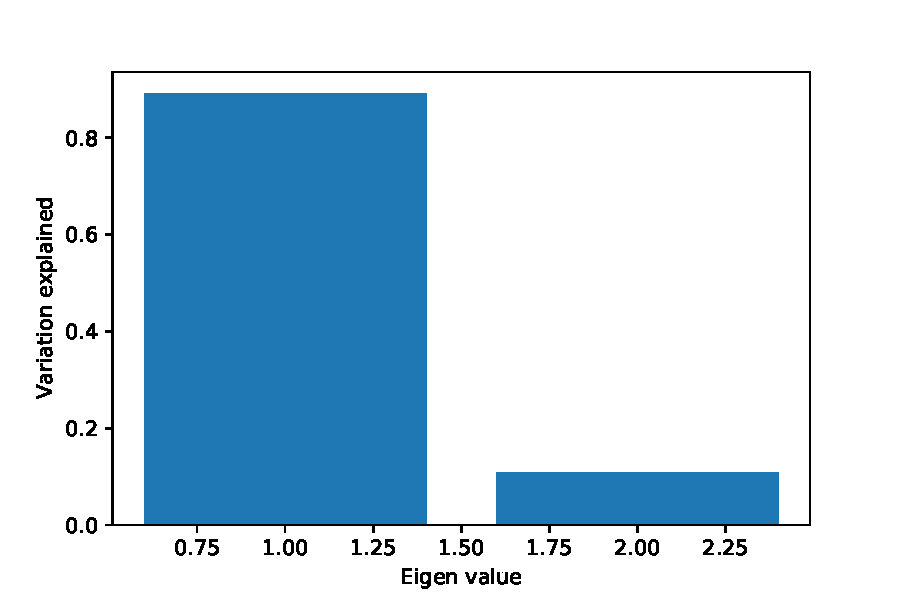
\includegraphics[scale=0.75]{media/profesores/barras.pdf}
\end{center}

\subsection{Proyectar los datos a una sola dimensión}
Como se dijo en el paso \ref{PCAmath-eigen}, Python hace todos los cálculos por nosotros, entonces ahora haremos una nueva instancia de la clase \texttt{PCA}, pero (a diferencia de antes) con solo una componente final.\\[0.75em]
\begin{minipage}[c]{0.48\textwidth}
Ahora vamos a realizar el producto punto entre el \textit{eigen vector} con \textit{eigen value} más grande y cada \textit{feauture vector} de los datos estandarizados.\\

En nuestro caso, $2.139$ con $(0.707, 0.707)$
\[ (0.707, 0.707)\cdot(-1.837,-1.643)=2.460 \]
y así sucesivamente.
\end{minipage}
\hfill\vrule\hfill
\begin{minipage}[c]{0.48\textwidth}
\begin{jupyter}{9}
pca3 = PCA(n_components=1)
pca3.fit(df_scaled)
Xpca3 = pca3.transform(df_scaled)
print("Projected data:")
print(Xpca3)
\end{jupyter}
\end{minipage}
\begin{table}[H]
\centering
\begin{tabular}{c}
\sffamily X projected \\ \hline
\rowcolor[HTML]{EFEFEF} 
$-2.460$ \\
$-0.820$ \\
\rowcolor[HTML]{EFEFEF} 
$0.045$ \\
$0.820$ \\
\rowcolor[HTML]{EFEFEF} 
$1.640$ \\
$0.774$
\end{tabular}
\caption{Datos proyectados}\label{tab:PCAmath-projected}
\end{table}
Cabe decir que en los últimos dos pasos los signos de los resultados están invertidos, esto no produce ningún cambio. Y con eso acabamos todos los calculos relativos a \textit{PCA}.
